\documentclass[a4paper]{memoir}
\usepackage[swedish, english]{babel}
\usepackage[T1]{fontenc}
\usepackage[sectionbib, round, authoryear, longnamesfirst]{natbib}
\renewcommand{\rmdefault}{pad}
\usepackage{graphicx}
\usepackage[a4paper]{geometry}
\usepackage{url}
\usepackage{setspace}
\onehalfspacing

% \lhead{\small{\textit{Henrik Frisk}}}
% \chead{}
% \rhead{\small{\textit{title}}}

% Different font in captions
\newcommand{\captionfonts}{\footnotesize}
\makeatletter  % Allow the use of @ in command names
\long\def\@makecaption#1#2{%
  \vskip\abovecaptionskip
  \sbox\@tempboxa{{\captionfonts #1: #2}}%
  \ifdim \wd\@tempboxa >\hsize
    {\captionfonts #1: #2\par}
  \else
    \hbox to\hsize{\hfil\box\@tempboxa\hfil}%
  \fi
  \vskip\belowcaptionskip}
\makeatother   % Cancel the effect of \makeatletter

\renewcommand{\figurename}{Fig.}

\title{Music, Computers and Interaction\\Introduction}
\author{Henrik Frisk\\henrik.frisk@mhm.lu.se\\Malm� Academy of Music,
  Lund University}
\date{\today}

\begin{document}
\selectlanguage{english}
\begin{titlingpage}
\aliaspagestyle{titlingpage}{plain}
\setlength{\droptitle}{40pt}
\maketitle
\vspace{5cm}

  \begin{minipage}[c]{\linewidth}
    \begin{center}
      \large{75\% seminar, December 10, 2007}
    \end{center}

  \end{minipage}

\vspace{5cm}

  \begin{minipage}[c]{\linewidth}
    \large{\emph{Opponent}:\\Prof. Simon Emmerson, DeMontfort Univ, Leicster,
    UK}
  \end{minipage}

\end{titlingpage}

\frontmatter
\settocdepth{subsubsection}
\tableofcontents
\listoffigures

\chapter{Preface}
\label{cha:preface}

This text and the collection of published papers, together form the
written part of my PhD thesis with the working title \emph{Music,
Computers, and Interaction}. The other two major parts of this work
are the artistic output\footnote{An archive containing all the
  material may be downloaded from
  \url{http://henrikfrisk.homeunix.net:8800/svn/dissertation/FriskMusic.zip}. 
Use `guest' for login and password. Should you experience problems
with the download, send me an email at henrik.frisk@mhm.lu.se. The
archive is nearly 700MB.} 
and the computer programs. Though a paper on the software project
libIntegra is included the software projects \emph{timbreMap} and \emph{libIntegra}
are not themselves included in this version of the thesis.

The main purpose of the first chapter (Chapter \ref{cha:introduction},
\emph{Introduction}) of this text is to provide the reader with an
overview of the research project. The next chapter (Chapter
\ref{cha:interaction}, \emph{Music and Interaction}) will discuss
interaction from a general, as well as to music specific
perspectives. Only the first part of Chapter \ref{cha:interaction} is
included in this version of the text. The first section (Section
\ref{sec:interaction} looks a differences between human-computer
interaction and social interaction as well as musical interaction and
in the first subsection (\emph{Social interaction and the giving up of
  the self}) I posit myself in the context of interaction. This
version of the text ends rather abruptly after this subsection.

What I intend for the continuation is a discussion of the parties
involved in any interaction from a subjective perspective, as `the
self' and `the other'. The next section will be an overview of the
field of interactive music, and finally a section about my own
interactive music. The final chapter, also not included here, will be
a summary and an outlook.

This is not the final version of any of the parts, but a version
produced for my 75\% seminar, the primary purpose of which is to `try
out' the material in the `real world'. I envision the final result of
this thesis to be produced in a hypertext format: The medium should
allow for seamless transitions between documentation of artistic
output and text based content. A somewhat evolved version of the way
the artistic output is presented.  (All material---text, music, and
programs---on a DVD browsable from a standard WWW browser.)
\clearpage
\section{Terminology and acronyms}
\label{sec:terminology}

Below is a list of terms that are used in these texts and that may
require some extra explanation.  Either because I want to delineate
its meaning or to avoid misunderstandings due to ambivalent
interpretations. Also included here are also acronyms
that, for the most part are explained in the text the first time they
appear.

\begin{itemize} %%% [\bfseries\textendash]

\item \textbf{ANN} - Artificial Neural Network.

\item \textbf{Agent} - In the studies performed within the frame of
  \emph{Negotiating the Musical Work} (see Section
  \ref{sec:negot-music-work}) we use the concept of `agent' (not to be
  confused with the software based `intelligent agent'). Many
  different kinds of agents are involved in the production of musical
  content. ``We find that by using the concept of `agents' we bypass
  the otherwise problematic values traditionally assigned to''
  `composer' and `performer' \citetext{see also \citealp[p.
    35]{wis96}}.

\item \textbf{Electro-acoustic Music} (EAM) - According to the Oxford
  English Dictionary electro-acoustics are ``acoustics investigated by
  electrical methods''\footnote{``electro-acoustics'' The Oxford
    English Dictionary. 2nd ed. 1989. OED Online. Oxford University
    Press. 31 Oct. 2007
    <http://dictionary.oed.com.ludwig.lub.lu.se/cgi/entry/50073014>}.
  Electro-acoustic music is a broad term used to denote music produced
  by or with electrical methods. Today, since this is mainly achieved
  by the use of digital computers, in USA the use of the term
  \emph{Computer Music} is more common\footnote{The issue of
    terminology in the field of electro-acoustic music is complex and
    there is an apparent lack of standardized vocabulary. How to
    label the entire genre, let alone sub-genres and particular
    processes within the field of electro-acoustic music, has recently
    been debated during a conference organized by EMS (see
    \citealp{EMS06}, in particular \citealp{landy06,dack06,battier06} and
    in relation to translation see \citealp{fields06}}). Yet another
  term, more commonly used in the francophone countries is
  \emph{acousmatic}, and it is sometimes argued that \emph{acousmatic}
  refers to the genre and \emph{electro-acoustic} to the means of
  production (e.g. \textparagraph 9 ``Vous avez dit...''
  \citeyear{musique-recherche}). In this text I will consistently use
  electro-acoustic music, or the acronym \emph{EAM} to denote my own
  artistic work involving computers and music.
   
\item \textbf{Esthesic} - An analysis of the (inductive) esthesic
  ``grounds itself in perceptive introspection'' - that which is
  ``perceptively relevant'', that which one hears \cite[pp.
  140-3]{nattiez}. See also \emph{Poietic}

\item\textbf{GUI} or \textbf{UI} - Graphical User Interface or User
  Interface.

\item\textbf{HCI} - Human Computer Interaction.

\item \textbf{Intelligent agent} - An idea to improve HCI introduced in
  the mid 90's. An agent is a piece of software designed to collect
  and sort information and present it to the user. The idea is that
  the agent will learn what it is its user wants, or needs to know
  about. (The `intelligent agent' should not be confused with the
  `agent' as a factor in the production of musical content.)

\item \textbf{Musician} - I use `musician' in a very inclusive
  way in these texts. A composer, an improviser, a performer are all
  sub-categories to the general description `musician'.

\item\textbf{Pitch-tracking} (also pitch-to-MIDI, pitch detection) - To
  let a computer (or a special purpose device) analyze an audio signal
  in real-time and extract the most likely fundamental of the
  sound. See the discussion i Section \ref{sec:interaction}. 

\item \textbf{Poietic} - According to musical semiologists Jean-Jacques
  Nattiez and Jean Molino, the poietic phase of a musical work is the
  stage at which the musical material is constructed. According to
  \citet{nattiez}, articulating the poietic and esthesic level
  ``facilitates knowledge of all processes unleashed by the musical
  work'' \cite[pp. 92]{nattiez}. We reinterpret the terms `poietic'
  and `esthesic' in the paper \emph{Negotiating the Musical Work} (see
  Section \ref{sec:negot-music-work}).

\item\textbf{Production of musical content} - Any or all activities
  involved when producing music - its conception, performance, writing
  down (transcription) and listening.

\item \textbf{SOM} - Self Organizing Map. A type of ANN introduced by \citet{kohonen88}.

% \item\textbf{Telematics} - ``Telematics is a term used to designate
%   computer-mediated communications networking involving telephone,
%   cable, and satellite links between geographically dispersed
%   indivudals and institutions that are interfaced to data-processing
%   systems, remote semsing devices, and capacious data-storage banks''
%   \citep[p. 241]{Ascott}

\end{itemize}

\section{Typography}
\label{sec:typography}

I have tried to follow the APA referencing guide for citations as
consistently and truthfully as possible except for references to the
Oxford English Dictionary where I have used the rules depicted by OED.
When citing in text I have put the reference after the closing
quotation mark but before the period. Quotes of 40 words or more are
inset and put in a separate paragraph and the reference is given
enclosed in parenthesis after the final period.

I use American style ``double'' quotation marks for quotes and
`single' quotation marks for inside quotes, except for longer indented
quotations. These are typeset without surrounding quotation marks and
any inside quotes are printed exactly as in the text cited. Commas and
periods are put inside the closing quotation mark, but colon and
semi-colon outside. Footnote marks are put after punctuation.

%%% Local Variables: 
%%% mode: latex
%%% TeX-master: "../MusicComputersInteraction"
%%% End: 


\mainmatter
\chapter{Introduction}
\label{cha:introduction}

\section{The research field and brief background}
\label{sec:research-question}

I do not believe that art is best created in solitary confinement but
that it is nurtured in social, human and cultural interaction. Whether
my background as a jazz musician and improviser is the explanation
for, or a consequence of this notion holds no real significance for
the reading of this dissertation, but there is an interesting
similarity between the sensibility required by an
improviser\footnote{I am referring to the kind of sensibility that
  George Lewis would refer to as \emph{afrological} \citep{lewis-1} -
  improvisation in which the personal narrative, manifested partly
  through the 'personal sound' is of importance and yet, in which the
  ''focus of musical discourse suddenly shifts from the individual,
  autonomous creator to the collective - the individual as a part of
  global humanity.'' (p. 110)} and the sensibility
required in any human interaction respectful of the other. 

The primary focus of my PhD project is the interaction between
musician and computer within the context of what is often referred to
as \emph{Interactive Music}
\citep[see][]{wiki_interactive,Garnett,rowe,winkler01,rowe01}. Though
this is a commonly used term its meaning is blurred by the magnitude
of concepts that it includes. Therefore in order to unwrap the idea
of musical interaction with a computer, the research project also
includes other forms for interaction in different contexts and between
other kinds of agents as well as different readings of the idea of
interaction. These investigations are conducted in the form of
reflection on my artistic as well as theoretical work. As we will see,
the consequences of the experiences gained from my practice as an
improviser and composer, may in the end change the way an interactive
system in which a computer is one of the agents, is designed,
approached and used. Hence, the study of musician-musician interaction
within this project is not a goal in itself but rather a way to
approach the complex field of musician-computer interaction. 

Although human-computer interaction (HCI from here on) is a very
active field of research, its results are not necessarily applicable
to the field of art practice. According to \citet{kuutti96} not even
software designers are making use of advances in HCI research: ``There
is a well-known gap between research results and practical design''
(p.  18). \citeauthor{kuutti96} is primarily looking at the
interdisciplinary research done in HCI and cognitive psychology and
concludes that ``some of the most remarkable new interfaces have been
developed with almost no help from research into cognitive
psychology'' (p. 18).\footnote{I should remark that a lot has happened
  in the ten years that has passed since \citeauthor{kuutti96} wrote
  this article and the surveys and references quoted are almost 20
  years old.} If the primary targets for HCI research---interface
designers and software developers---are not finding use for it, what
is in it for the arts?

This is not to say that HCI research is useless---on the contrary---it
is a very important research field with an ever increasing number of
applications. But, what is HCI? What does it mean to interact with a
computer?

\subsection{Human-Computer Interaction: HCI}
\label{sec:human-comp-inter}

\citet{thomassen03} offers the following perhaps self-evident general
definition: ``Interaction involves two participants: the user and the
computer.  The interaction is aimed at supporting the user to
accomplish the goals set by a specific application \textit{domain}''
(p. 105, italics of the author). A similar account is given by
\citet{clubb07}: ``HCI deals with design for ease of use and making
the interaction with the computer system as user-friendly as
possible'' (p. 35). In other words, the idea of HCI is to help the
user accomplish a task and the result of the design effort that is
initiated by HCI is the User Interface (UI). The UI is the layer of
mediation between the user and the computer. Metaphorically, if the
computer is a hammer, the UI is the grip that allows the user to use
the hammer without dropping it and the activities that led to the
design of the grip of the hammer \emph{and} the usage of the hammer is
what would correspond to HCI. Looking at it from this angle makes it
appear as a methodology of control---of curbing the powers of the
machine. In particular in commercial operating systems design, the
purpose of the UI is to conceal the complexity of the computer to the
user. The Graphical UI (GUI from here on) and the desktop metaphor
became a very popular and celebrated mediator for HCI when the first
personal computers became commercially available in the 70's and, in combination
with the advent of the mouse, has come to dominate the way we interact
with computers. In the book \emph{Interface Culture - How new
  technology transforms the way we create and communicate} gives
(among other things) an excellent historical overview of the
development of the GUI of the modern computer operating system
\citet[chap. 2 \& 3]{johnson97}.

A significant feature of a GUI is the use of icons as a replacement
for text---rather than typing text based commands on a terminal we
click on an icon that represents the operation we want the computer to
perform. Neal Stephenson takes position against this focus on the
\emph{icon} and the visual forms of communication in the modern GUIs
which he compares to the illusive appearances offered at Disney World:
``Disney is in the business of putting out a product of seamless
illusion---a magic mirror that reflects the world back better than it
really is'' \citep[p. 50]{stephenson99},\footnote{A similar account is
  given by Umberto Eco in his essay \emph{Dalla periferia dell'impero}
  (\emph{In the heart of the empire}). In the chapter
  \emph{City of the robots} (my trans.) Eco is comparing the
  experience of watching the illusory machinery of Disneyland, the machine
  alligators, to the real thing as watched (but not seen) from a boat
  on Mississippi River reaching the conclusion that the perfect
  execution and predictability of Disney's robots give them a far
  higher entertainment value: ``By Disneyland we are told that
  technology can give us much more than nature'' \citep[p. 53]{eco87}}
and he concludes:

\begin{quote}
  Disney and Apple/Microsoft are in the same business: short-circuiting
  laborious, explicit verbal communication with expensively designed
  interfaces. Disney is a sort of user interface unto itself---and more
  than just graphical. Let's call it a Sensorial Interface. It can be
  applied to anything in the world, real or imagined, albeit at
  staggering expense. (p. 52)
\end{quote}

Not only do I not believe that computers of today are properly
signified by the notion of a `tool', neither are concepts such as
`concealing complexity', `control' and `ease-of-use' especially useful
in my musical practice---in particular not in improvisation. I don't
think of my saxophone as a tool, neither do I want my computer or any
of the technologies I use in my artistic practice to be merely
`tools'. Whatever machinery is used and needed in the process is as
much a part of the artistic work as are any performers participating.
Together they form the social---and, in a wider sense of the word, the
technical---context in which performing and, hence communication,
takes place. I will do the best I can to \emph{not} attempt to control
or restrict the powers of my co-musicians, nor do I want them to
conceal the complexity of their behavior. Neither do I want a computer
interface in the context of my artistic practice that has been
curtailed in order to improve someone else's notion of
user-friendliness.

Ideas along the same lines, though for different purposes, seem to
be getting some support from authors \citeauthor{krilik04} who, at the
very end of their paper about ``[a] common framework for studying
perception and performance in both human-technology interaction and
music'' (p. 616) brings in improvisation in the discussion of
Sociotechnical Systems:
\begin{quotation}
  Currently, however, our experience is that design and
  training in many sociotechnical systems proceed all to often
  as if `doing it by the book' or working `like a machine'
  were admirable qualities. Experienced human operators
  know otherwise, and in their better moments, so do engineers,
  researchers and practitioners in human-technology
  interaction. Investigations of the constrained liberation
  underlying musical performance may hold promise for the
  development of a theory of responsible improvisation that
  could have significant social value. \citep[p. 629]{krilik04}
\end{quotation}
In the already mentioned PhD dissertation on using the \emph{flow}
heuristic when building GUIs for web based applications,
\citeauthor{thomassen03} mentions music as means``to fully research
the applicability of the heuristic.  The major disciplines are the
field of social sciences such as psychology and cultural studies, but
also the field of the arts in particular music and fine arts''
\citep[p. 239]{thomassen03}.

Technology as well as art is constructed by how we think about it. I
acknowledge the need for the average computer users to have a UI that
makes their interactions easy and effortless.\footnote{It should be
  noted that I don't think that this stage is by far reached in the
  operating systems and programs offered by commercial companies
  today. In a big survey (6.000 participants) produced by one of the
  largest national trade unions for officials in Sweden (Sif), though
  80\% felt the IT systems used where invaluable in their day to day
  work and in their customer relations, a stunning 50\% felt the
  software negatively influenced the way they worked, and 50\% felt
  the interfaces and help functions were defective (bad usability)
  \citep{sif07}.}  But those needs, and the thinking and research that
has led to the solutions of the problems addressed by those needs, is
not necessarily useful when we move from the domain of production and
corporate efficiency to the abstract domain of artistic practice. That
the latter domain has been used to inform or inspire the design of a
UI, as \citeauthor{thomassen03} and \citeauthor{krilik04} suggest
should be done, will in this regard not make a decisive difference.
When interacting with a computer in the context of (improvised) music
questions regarding the interaction---its prerequisites and its
needs---are raised. The questions may be asked looking at the matter
from the `outside' (I can never be completely outside my own artistic
practice) or they may be asked investigating the object from the
`inside'. The questions will not always be the same ones but will vary
along with context and with time, just as the needs imposed on the
interaction will not be the same for every situation. This research
project is about defining and posing these questions from the
standpoint of my artistic practice.

\subsection{Personal background}
\label{sec:personal-background}

For me as a musician, I have two principal areas of interest:
\renewcommand{\labelenumi}{\arabic{enumi}}
\begin{enumerate}
\item \textbf{Improvisation}. As a performer I look at different ways
  to explore improvisation: Idiomatic (primarily jazz) as well as
  non-idiomatic,\footnote{These terms, `idiomatic' and `non-idiomatic'
    are borrowed from Derek Bailey \citep[see][]{bailey92}}
  pre-structured and without preparation (as little as is possible),
  on acoustic instruments and on electronic and home made instruments
  (mostly software instruments on laptop). Even when working with
  composition in a relatively traditional manner (i.e., using musical
  notation), I am always looking for ways in which the score can adopt
  an open frame of reference for the performer to adjust to his or her
  will.
\item \textbf{Computers}. I have worked with the computer in one way
  or another in almost all of my artistic work since 1994. As an
  artist I feel a responsibility to explore the world and its
  artifacts. The computer has become an important part of this world
  and hence, a part of our culture. In the Western world it is part of
  daily life and allows for our most basic as well as our most
  intimate communications. It cannot be placed outside of our culture,
  nor can it be regarded as merely a tool or a fashionable gadget with
  a limited import; rather it must be included in our understanding of
  the world as well as in our artistic explorations.
\end{enumerate}

My interest in integrating and interacting with electronically
produced sounds began in the late 80's when listening to saxophonists
such as Gary Thomas \citep{thomas88} and Greg Osby
\citep{dejohnette88} using the IVL Pitchider\footnote{The IVL
  Pitchrider is now out of production. At its time it was a state of
  the art pitch-to-MIDI converter. It took an audio signal from a
  microphone and send out a MIDI signal that could be used to control
  a synthesizer (see also the terminology in Section
  \ref{sec:terminology}.} and Frank Zappa playing the Synclavier
\citep{zappa86,wiki_synclavier}. Pat Metheny's use of guitar
synthesizer and sampler on the \emph{Song X} record, together with
Ornette Coleman, was a thrilling sonic experience of what could be
done with, what we today would call relatively simple, technology
\citep{metheny86}. Later, hearing George Lewis's \emph{Voyager}
\citep{lewis92} I realized the possibilities for something else than
the one-to-one mapping between the instrument and the
electronicsused in the examples above,\footnote{To be honest it was already when listening to
  the track \emph{Traf} on Gary Thomas' \emph{Code Violations} that I
  started thinking about different mapping schemes inspired by Gary
  Thomas: ``I assigned a different harmony note to each note I play on
  the saxophone; I set it up the way I prefer to hear notes run
  together'' \citep[Cover notes, \textparagraph 7]{thomas88}. In the
  same text Thomas makes another interesting remark that had a big
  impact on me: ``You can take the limitations of tracking technology
  and turn them into advantages: if you bend a note on the sax, the
  synth note doesn't bend, so you get some dissonances'' (\emph{ibid}
  \textparagraph 7).  The idea of using the limitations of technology
  to ones advantage had a big impact on me.} later described by
\citeauthor{lewis00} as ``I conceive a performance of Voyager as
multiple parallel streams of music generation, emanating from both the
computers and the humans---a nonhierarchical, improvisational,
subject-subject model of discourse, rather than a stimulus/response
setup'' \citep[p. 34]{lewis00}.

In the early 90's I was not attached to any academic music institution
and I had no computer science training or knowledge. What started at
this time was a long process of \emph{reverse-engineering} the sounds
I had heard and the processes I was interested in, in total absence of
a terminology or even language in which to express what I wanted to
achieve. The only method available to me was trial and error. In a
sense, this thesis is the collection of information, reflection, and
documentation that I would have liked to have access to at the time of
my first steps in \emph{Interactive Music}. In hindsight I can see
that a lot of material, experience and expertise existed but my lack
of knowledge and terminology, in combination with my personal and
artistic preconditions, made it necessary for me to begin by finding
out by myself.

\section{Summary of the research field}
\label{sec:summary}

Obviously (hopefully), I have since come a long way and the current
PhD project marks an important step in the work in progress for which
the goal may be summarized as: To be able to dynamically interact with
a computer in my own improvised performances as well as allow for
other musicians to similarly interact dynamically with a computer when
performing my music. `Dynamically' should be understood as non-static
in the moment of performance, i.e. real-time dynamic, but also dynamic
with regard to context in non real-time: To not accept one particular
solution but to constantly re-evaluate and search for that which each
situation requires.  This idea of `dynamic' also relates to the
re-evaluation of `the self' in \emph{any} musical interaction and
production of musical content. And in this thesis, specifically, I
will investigate how the concept of `giving up of the self' as the
first step of human-human interaction on equal terms may be applied to
human-computer interaction in the context of production of musical
content.

% In Section \ref{sec:interaction} I will discuss \emph{Interaction} in
% general and then, in Section \ref{sec:interactive-music} I will look
% at that which is commonly referred to as \emph{Interactive Music}.
% That being the meta-level of interaction, I will then proceed to
% discuss the micro-level, the code, or the language and the processes
% of signification---and its nature and quality---and if that may or should
% be considered in interactive music.

Though this thesis marks the end of one phase it most certainly, for
me personally, marks the beginning of another.

\section{Overview of contents}
\label{sec:overview}

Although I prefer to see all aspects of this PhD project as a
distribution of interrelated parts all belonging to my artistic
practice, I acknowledge the need for a structure in which the reader
can navigate the contents. This section is intended to be an
annotated table of contents for the reader to get an
overview of the project but also to allow for reference look-up of a
particular component.

\begin{figure}[!hb]
  \centering
  \includegraphics[width=0.9\textwidth]{img/project-overview2}
  \caption{The three main components of the dissertation and their
    relative position in an imaginary field of practice.}
\label{fig:project_overview}
\end{figure}

\subsection{Artistic Output (music)}
\label{sec:artistic-output}

In this project the artistic work is, in a sense, both the object and
the method. These projects, some of them still works-in-progress, are
used to make inquiries into the larger question of the significance of
interaction in the context of artistic practice. They are
manifestations of different modes of interaction and as such they form
the stipulation for the reflections on interaction presented. But they
are also carriers of artistic experience and as such they have in
themselves something to say about the subject matter.

The different modes of interaction represented in these artistic
projects are not only relating to musician-computer interaction but
also, to a high degree to musician-musician interaction: Interaction
taking place in the stages of preparation and development of the
projects as well as in the processes of performance, execution and
evaluation.


\subsubsection{Drive (2003)}
\label{sec:drive-2003}

\emph{Drive} is a composition for Electric Viola Grande
(EVG)\footnote{The Electric Viola Grande is a custom made,
  electronically amplified five stringed viola. It was built by
  Swedish instrument builder Richard Rolf on commission from Swedish
  violist Henrik Frendin.}  and computer commissioned by Swedish
violist Henrik Frendin for his Phono Suecia recording \emph{Viola con
  Forza} \citep{frendin04}. Within the frame of the composition the
performer has a lot of freedom to shape the piece in a way that he or
she sees fit in order to fulfill the larger structural idea of the
composition: a dominant to tonic cadence. Its interaction scheme is
based on the widely used space-bar-piece paradigm\footnote{I heard
  this term used for the first time by Sean Ferguson (see
  <\url{http://www.cirmmt.mcgill.ca/People/ferguson}>). In the mid
  90's when it started to become practical to use computers in
  live performance a large number of compositions where produced where
  someone other than the performer(s)---usually the
  composer---interacted with the computer using the
  keyboard. Each press on the space bar started the playback of the
  next pre-prepared sound file or changed a preset for an effect or a
  synthesizer or whatever the next `event' required. It is still a
  very common mode of interaction in the electro-acoustic music
  community.}: The computer is stepped through the different sections
of the form of the composition by giving it cues (pressing the space
bar).\footnote{The cue may of course come from any kind of control
  source from which a clear, noise-free, trigger can be generated - a
  pedal pressed by the performer, a uniquely detected pitch in the
  audio signal, a change of volume, etc.}  However on a lower level
its interaction with the musician is fairly dynamic as all sounds
produced by the computer are 'filtered'\footnote{Filtered as in
  spectrally mutated but also in a more symbolic sense of the word.}
by the sound of the EVG. In that sense the role of the computer is
that of a virtual resonance that is used to expand the spectral range
of the instrument.

Apart from being an example of a fairly standard way of working with
interactive electronics, \emph{Drive} is a composition in which the
interaction between myself as the composer and Henrik Frendin as the
interpreter is mediated through an open ended score. We both have to
question our respective views and personal wishes and open ourselves
up to the other's point of view and trust that that view is `genuine'.

\subsubsection{etherSound (2003)}
\label{sec:ethersound-2003}

\emph{etherSound} is perhaps the most ambitious project within my PhD
project. It investigates many of the aspects of the research
question and may perhaps best be described as an environment
that allows for interaction between different agents on different
levels simultaneously. It takes input in the form of SMS messages sent
from a mobile telephone and transforms the text of the message to a
sound event that lasts between a few seconds up to over a minute. The
length and complexity of the sound event is governed by the length and
complexity of the current input as well as of previous input. 

I review this project and examine the various ways in which
interaction is taking place within it as well as give a description of
the inner workings of it. Audience participation is an important
aspect of \emph{etherSound} and may distort the way we understand the
roles of the agents involved in the production of this event. Further,
this relates to the discussion of the ontology of the musical work
which is being probed in the paper \emph{Negotiating the Musical Work.
  An empirical study on the inter-relation between composition,
  interpretation and performance.} (see Section
\ref{sec:negot-music-work} and also \citet{frisk-ost06}).

\subsubsection{Solo improvisations (2002-2007)}
\label{sec:solo-impr-2002}

It is within my work with solo saxophone and computer improvisations
that I will be able to assess the particular validity of the study of
musician-computer interaction. And it is in this context that I will
articulate that which I reach for in interactive saxophone-computer
improvisation.

\subsubsection{Frisk/Nilsson duo (2005-2007)}
\label{sec:friskn-duo-2005}

Within the context of my duo performances with Per Anders
Nilsson\footnote{Per Anders is also a PhD student within the field of practice
  based research in music. He is doing a joint degree between
  the Department of Musical Interpretation and Performance at the
  Academy of Music and Drama at G�teborg University and Dep. De
  Communicacao E Arte at Universidade de Aveiro, Portugal. The focus of his
  project is the computer as a musical instrument.} we have
experimented with fairly complex interaction schemes and feedback
processes. Per Anders has developed unique computer based instruments
as well as methods with which to perform on these. This allows for an
interesting possibility for me to investigate how, if it is a human
mediating the interaction between my saxophone playing and the
computer playing or computer based alteration of the saxophone sounds,
the result may differ from my solo work in which I attempt to
pre-model the activities of the computer. And further, what is the
difference between interacting musically with a musician playing the
computer and a musician playing an acoustic instrument? 

\subsubsection{Repetition Repeats all other Repetitions (2006)}
\label{sec:repet-repe-all}

This collaboration with the Swedish guitarist Stefan �stersj� is an
example of a project in which already at the outset interaction was
allowed to play a major part. Though the project is fairly well
documented in the article \emph{Negotiating the Musical Work. An
  empirical study on the inter-relation between composition,
  interpretation and performance.} (see Section
\ref{sec:negot-music-work} and also \citet{frisk-ost06}), just as with
\emph{etherSound} I will review our findings. What is the difference
between this form of interaction and the kind of interaction that takes
place in \emph{Drive}? The computer part is more of a counter
point to the instrumental part in this piece than in most of my other
work for instrument and computer. What effect does that have on the
way the performer-computer interaction is achieved?  Together, myself
and Stefan have produced and performed two different versions of this
piece and we attempt to prepare a third version to be premiered in May
2008. This third version will take account on the ideas that were
developed building on the experiences from the two first versions,
primarily regarding the interaction between Stefan and the computer.

As with \emph{Drive} this project is also an example of how the
interaction between myself and Stefan is allowed to influence many
aspects of the music. Perhaps more radically and far-reaching
here than in my previous projects, considering the thorough
preparative studies we performed together.

\subsubsection{The Six Tones (2006)}
\label{sec:six-tones-2006}

\emph{The Six Tones} is a composition for two traditional Vietnamese
instruments Dan Bau, Dan Tranh, banjo and 10-stringed guitar, and
computer. This too is a close collaboration, this time between myself,
Stefan �stersj� and two Vietnamese master musicians Nguyen Than
Thuy and Ngo Tra My. We met for the first time in April 2006 and
started improvising on some sketches I had made. Not only were these
improvisations later used to compose this piece, some of the
improvisations were also transcribed and used in \emph{Repetition
  Repeats all other Repetitions}. One of the interesting aspects of
this project in relation to the main research topic is the limited
possibilities for verbal interaction that is a result of the language
barrier.

Apart from the composition \emph{The Six Tones} we also performed
versions of traditional Vietnamese music in which I participated on
laptop. It forms an example of inter-cultural musical interaction in
which style and idiom are radically mixed and altered.

\subsubsection{Piece for harp and computer (2008)}
\label{sec:piece-harp-computer}

Though this piece has been in the workings for several years it will
not be premiered until 2008. Its interaction scheme will be based on
the timbreMap software.

\subsubsection{Piece for small ensemble and speakers (2008)}
\label{sec:piece-small-ensemble}

This piece is a commission from \emph{Copenhagen Art Ensemble}. It
will be premiered in May 2008.

\subsection{Computer programs (software)}
\label{sec:tools-programming}

The computer software---programs and libraries---built and included in
this project are not merely ``tools'' to allow for ``testing''. I
regard them as part of the artistic practice that lies at the very
foundation of this project, i.e. they are implementations of ideas,
but they are also beginnings in themselves in that they may, albeit in
a limited sense, allow for a different usage of computers in the
context of interactive music. The purpose of my PhD thesis is not to
draw conclusions that may be \emph{generalized} and used in other
contexts but rather to test assumptions within the framework of my own
artistic production. However, the software tools, released under the
\citet{GNUGPL}, may very well be used in other contexts, by other
artists for completely different purposes, or to further elaborate on
the ideas presented in this thesis.

\subsubsection{timbreMap}
\label{sec:timbremap}

The \emph{timbreMap} software is an attempt to assess the hypothesis
that the relation between the nature of the signal used in the
musician-computer interaction is of importance. It makes use of the
JetNet \citep{lonnblad91} library implementation of neural networks
and processes real time audio to extract feature vectors that are fed
into a Self-Organized Map (SOM), as it is described by
\citet{kohonen88}, that maps changes in the input vectors to a 2D
feature space.

I will experiment with \emph{timbreMap} as a complement to a
pitch-tracker. With it I will be able to inform the computer of
relative changes in timbre and this, I hope, will allow me to further
expand on the possibilities for musician-computer interaction. It is
the attempt at addressing the issue discussed at the end of Section
\ref{sec:music-pract-inter}.

\subsubsection{libIntegra}
\label{sec:libintegra}

Integra \citeyearpar{integra-web} is a EU Culture 2000 pan-European
artistic and scientific project. One of the goals is to develop a
composition and performance environment for sharing live music
technologies. One part of that environment is the Integra library
(\emph{libIntegra}) which is also included in my thesis. It is a set
of software tools that allow many musicians to interactively work on
many different kinds of collaborative projects in a way that have not
been possible earlier. 

\emph{libIntegra} allow for a standardized way of representing and
storing parameter spaces for multi-media modules.  One of the things
this allows for is seamless interchange of units of DSP processing
(software or hardware based) within a given context. A performer that
wants to improvise with an environment that requires a Yamaha DX7
synthesizer may simply substitute the hardware with a software
representation of the same synthesis model. As long as the
environment, and the modules within it, comply with the Integra
standard the exchange is transparent from the user point of view. The
library is also able to interface with a centralized database and
versioning server making interaction on any kind of content that the
database and the library may represent easy and, in that sense it is a
software representation of the very idea of the musical work as a
result of distributed actions in continuous interaction.

\subsection{Published papers (text)}
\label{sec:reflections-text}

\subsubsection[New communications technology...]{New communications
  technology in the context of interactive sound art: An empirical
  analysis. \citep{frisk05}}
\label{sec:new-comm-techn}

Co-written with my former colleague Miya Yoshida, the curator who
originally commissioned \emph{etherSound}, this article is mainly
focused on aspects of collaborative artworks. We discuss the notion of
`interaction' and `participation' and `the public' and, since
\emph{etherSound} at this stage was very much a collaboration between
myself and Miya, the text is in itself an example of artistic
inter-disciplinary interaction.

The transformation from private to public in \emph{etherSound} (an SMS
emanating in the private sphere from a privately owned mobile phone
results in a publicly perceptible sound event) opens up for a new
sensation of space and an auspicious and dynamic impression of
creativity. This shift, from private to public is related to the, for
this thesis central idea of `giving up of the self' (the private) as a
first step to interaction (the public) on equal terms. Further we look
at new communications technology in the context of art production and
come to the conclusion that particularly the mobile phone may (i) be
successfully incorporated in collaborative art, (ii) has advantages as
compared to other, similar, technologies.

\subsubsection[libIntegra]{libIntegra: a system for software-independent multimedia
  module \citep{frisk-bull07}}
\label{sec:libint-syst-softw}

The main interest of the libIntegra project in relation to my thesis
is its implications concerning the notion of the musical work, as the
software allows for seamless integrated documentation of many
different kinds of musical works---scores, interpretations of scores,
performances of scores, improvisations, improvisation environments,
etc.. \emph{libIntegra} also allows for interaction across computer
platform boundaries and with it \emph{timbreMap} integrates with any
other software for which \emph{libIntegra} has support. The paper is
co-written with Jamie Bullock at UCE, Birmingham Conservatoire,
department of composition. It describes the structure of the software
library referenced above (\ref{sec:libintegra}). This too is a
collaboration, however of a somewhat larger scope\footnote{Though
  myself and Jamie Bullock are the main developers of the libIntegra
  software, the project Integra has members from 11 countries and 6
  universities and there is a total of 10 research centers and five
  new music ensembles involved.}.


\subsubsection[Negotiating the Musical Work]{Negotiating the Musical Work. An empirical study on the
  inter-relation between composition, interpretation and performance. \citep{frisk-ost06-2}}
\label{sec:negot-music-work}

The purpose of the studies described in the article is to explore the
inter-relations between performer and composer. Specifically we study
the musical work in the Western art music tradition, prior to its
ultimate notation and prior to its performance. We present a method
with which studies on the low level processes in the production of
musical content may be performed drawing on semiological thinking.
Following a discussion of the ontology of the musical work and the
function of musical interpretation we claim that: (i) Musical interpretation can be divided into
two kinds: `thinking-through-practice' and analytic (critical)
interpretation. (ii) Interpretation plays a crucial role in the
practice of both the composer and performer. The method presented is
applied in a study described in another article which is not part of
this thesis but which I will briefly summarize here \citetext{see
\citealp{frisk-ost06}}. 

In an analysis of a video recording of the collaboration between
Stefan �stersj� and composer Love Mangs we draw the conclusion that,
rather than being a one way constructive process ``composition may be
regarded as a complex interaction between esthesic and poietic
processes''. In the analysis of the performer-composer interaction we
note that ``[t]he flexibility [...] in the interaction between the
two agents in the video clip is remarkable. Complete misunderstandings
and miscommunication does not halt the process nor does it appear to
lead to false conclusions''. We further look at ways in which the
knowledge gained from analyzing the collaboration may be used to
inform the design of an interactive interface for a mixed media
piece to be performed live and we draw the following, somewhat
pointed, conclusions:
\begin{itemize}
\item Noise in communication may not be a problem.
\item Direction may be more important than synchronicity.
\item The initiative may shift independently of the esthesic and
  poietic processes.
\end{itemize}

Both of these articles are a result of my collaboration with
Stefan �stersj�, that preceded the composition
\emph{Repetition Repeats all other Repetitions} (see Section
\ref{sec:repet-repe-all}). Our collaboration in the preparatory stages
of the process of composition allowed us to enter the project with a
slightly different view on our respective practices that, in
hindsight, I am certain has had a very positive effect on my own
artistic practice in general.

\subsubsection[etherSound]{etherSound - an interactive sound installation \citep{frisk1}}
\label{sec:ethers-an-inter}

If the essay \emph{New communications technology in the context of
  interactive sound art.} (see Section \ref{sec:new-comm-techn}) dealt
with the \emph{etherSound} (see Section \ref{sec:ethersound-2003}) in
the context of the visual arts---as an installation---this article is
more focused on the performative aspects of the project within a
musical context. The design of the current and previous versions of
\emph{etherSound} (see section \ref{sec:ethersound-2003}) is explained
and the synthesis and sequencing algorithms---the text to sound
transformations---are discussed. In the frame of my research project
as a whole, \emph{etherSound} is perhaps the most distinct example of
the artistic practice as both object and method. The problematic
relation between user \emph{control} through interaction---the
participant's chance to discriminate his or her input from other
input, i.e. the transparency of the system, and interaction
as `dialog' is further discussed.

At the end of the paper on performer-composer interaction summarized
above \citep{frisk-ost06} we make a note that the main difference
between the activities of the two agents is the intention: ``The way
the idea of the composer has been deconstructed in this study, what
remains of it is 'the one with the intention to create' ''. This is
related to \emph{etherSound} in that the wish to participate is
intended to be the only requirement for participation: The audience is
used (exploited?) to supply that which the computer does not have (and
which we are not likely to be able to model within a computer for many
years still)---intentionality.

\subsubsection[timbreMap]{timbreMap - using a Kohonen net for tracking relative
  timbre changes in an audio signal in real time. (not yet published)}
\label{sec:timbr-using-kohon}

Work in progress. Unpublished.

\section{Artistic practice and interaction---Summary}
\label{sec:music-pract-inter}

To summarize, the different types of interaction, or contexts in which
some interaction takes place, dealt with in this research project,
explicit in this or related texts, or implicit in the artistic or
programming projects included, are:
\begin{itemize}
\item \textbf{Musician-Computer Interaction}
  \begin{itemize}
  \item Performer-computer interaction in score based works
    (\emph{Drive}, \emph{Repetition...}, \emph{Harp piece}, \emph{timbreMap})
  \item Performer-computer interaction in improvised works (\emph{solo
    improvisations}, \emph{timbreMap})
  \item Performer-computer interaction in laptop
    performance. (\emph{The Six Tones})
  \end{itemize}
\item \textbf{Musician-Musician Interaction}
  \begin{itemize}
  \item Composer-performer interaction (\emph{Repetition...},
    \emph{The Six Tones}, \emph{libIntegra})
  \item Performer-performer interaction (\emph{Frisk/Nilsson Duo})
  \item Performer-audience interaction (\emph{etherSound}, \emph{libIntegra})
  \end{itemize}
\end{itemize}
Each type of context has its own set of requirements. A performer
playing a scored piece for instrument and computer have different
needs and expectations than does an improviser, and all performers do
not have the same anticipations. Improvising \emph{with} a computer as
a saxophonist is in every respect different from improvising \emph{on}
the computer. If this delineates the contexts in which subjects
interact, the nature of the interaction, its character, either achieved or
attempted at, I will address in the following paragraphs.

In his book \emph{Interactive Music Systems}, composer, programmer,
and researcher Robert \citet{rowe} makes a classification of
interactive music systems that may prove useful to help determine the
purpose, or the objective, of these eight projects---containers of
musical practice---within the context of the larger scope of the
research project as a whole. I will apply these classifiers, partly to
assist the reader as a complement to listening, but also in an attempt
to dismantle the concepts involved, as part of the research: ``This
classification system will be built on a combination of three
dimensions, whose attributes help identify the musical motivations
behind types of input interpretation, and methods of response'' (p.
6). Finally, it will provide us with a terminology which can be used
to ``distinguish and draw relations between interactive programs'' (p.
7).  Though \citeauthor{rowe} uses the classifiers primarily for
computer \emph{programs} I find them useful also for the point at
issue.\footnote{This is likely to be because most of these projects
  feature at least one `program', specially designed for the purpose,
  even though it may only consist of a simple Max patch \citep{max}.}

The categories in the three dimensions are: 

\begin{enumerate}
\item \emph{Score-driven} systems versus \emph{performance-driven},
  i.e.  systems that range from ``programs that use predetermined
  event collections'' (a score), to those that ``do not anticipate the
  realization of any particular score''.

\item \emph{Transformative}; that apply a transformation on some
  existing material, \emph{generative}; that generates material from
  ``elementary of fragmentary'' source material (a scale or a chord),
  or \emph{sequenced}; that ``use prerecorded music fragments'',
  response methods.

\item \emph{Instrument}; ``concerned with constructing an extended
  musical instrument'', and \emph{player}; concerned with constructing
  ``an artificial player'', paradigms (p.  7-8).
\end{enumerate}


\begin{figure}[!htb]
  \centering
  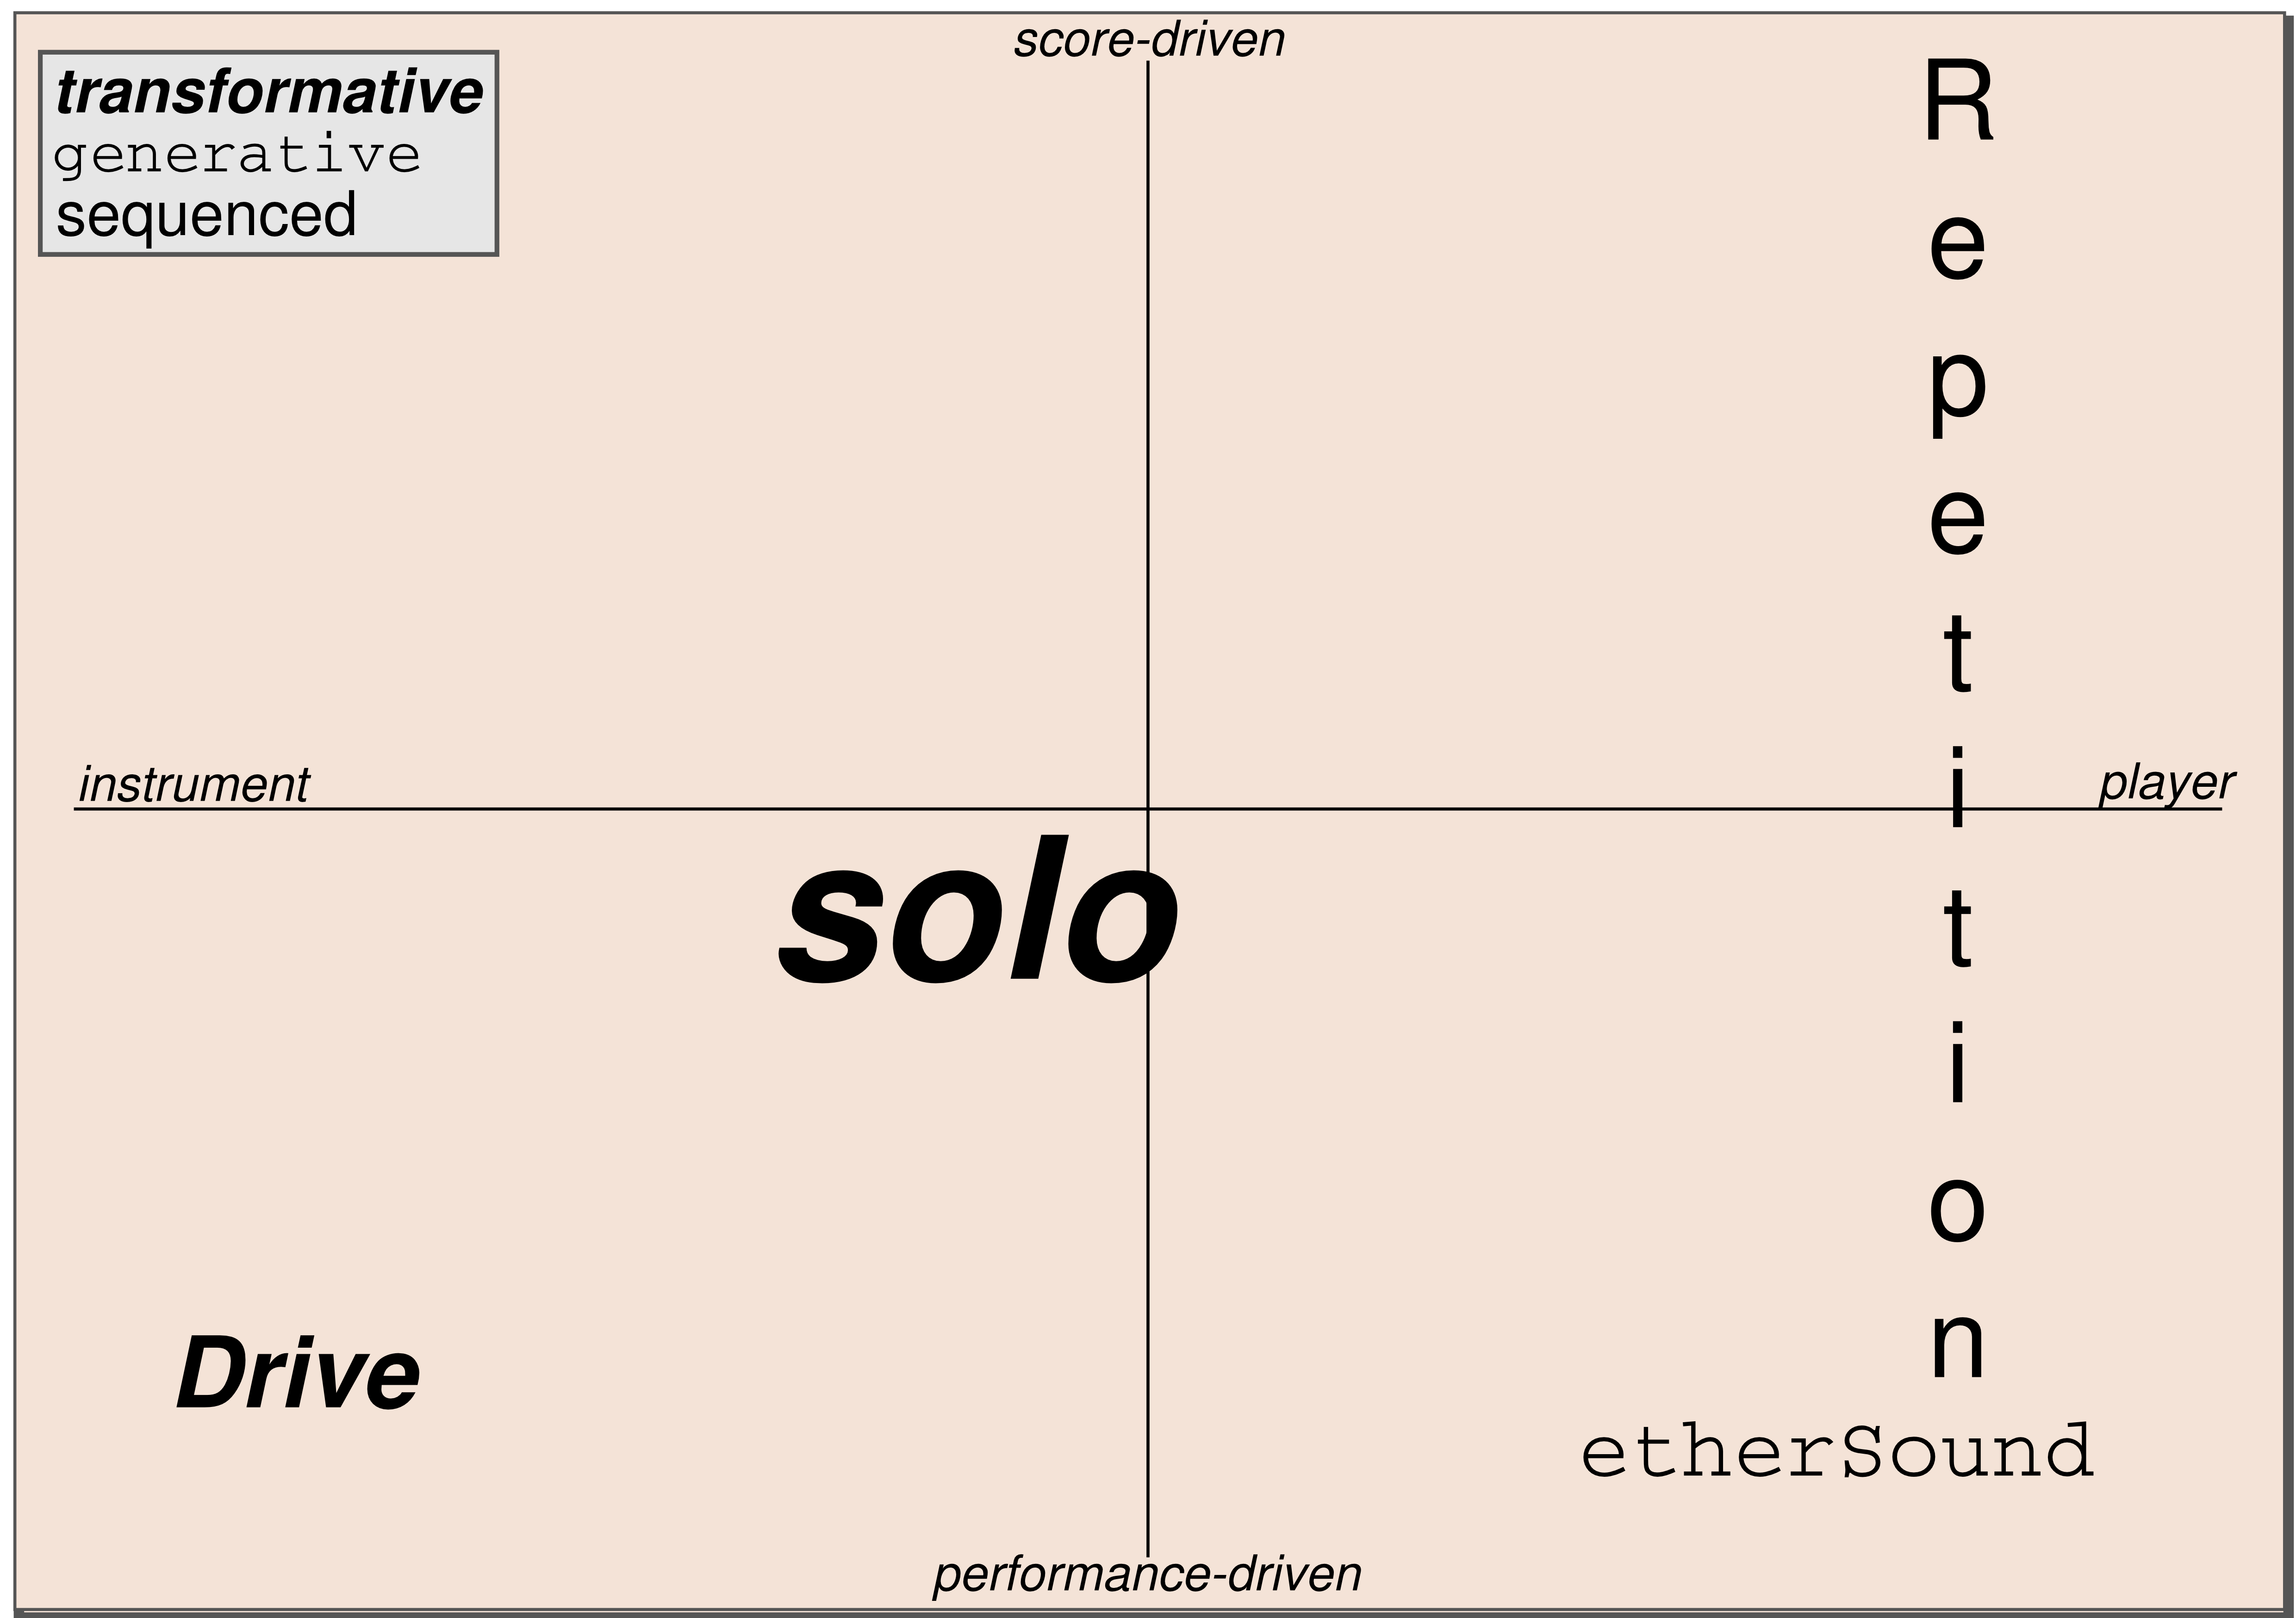
\includegraphics[width=0.9\textwidth]{img/interact-class}
  \caption{The approximate position of the artistic content in the three
    classification dimensions suggested by \citet[p. 5-8]{rowe}. The font \textit{type}
  is used in the graph to discriminate between the different response
  methods. The font \textit{size} I have used to indicate the stability of the
  project in relation to the categories. For example, in the
  \emph{Frisk/Nilsson Duo} we use a large number of interactive
  techniques and programs, hence the font size is large, whereas
  \emph{Repetition Repeats all other Repetitions} is fairly well
  categorized as a score-driven system employing a player paradigm with
  predominantly sequenced response methods---and is thus represented with
  a small font size.}
\label{fig:interact-class}
\end{figure}

Following is a suggestion of a classification of the pieces included
in this thesis, using Rowe's categories:

\begin{itemize}
\item All except \emph{Repetition Repeats all other Repetitions},
  \emph{Piece for harp and computer} and \emph{Piece for small
    ensemble and speakers} employ (or will employ) performance-driven
  systems.
\item \emph{Drive}, \emph{Frisk/Nilsson Duo}, \emph{Piece for harp and
    computer}, \emph{The Six Tones}, \emph{Piece for small ensemble
    and speakers} and my solo improvisations use primarily
  transformative response methods. \emph{etherSound} use generative
  and \emph{Repetition Repeats all other Repetitions} use sequenced
  response methods.
\item \emph{etherSound}, \emph{Repetition Repeats all other
    Repetitions}, some of my solo improvisations and \emph{The Six
    Tones} are versions of the player paradigm, the rest follow more
  of an instrument paradigm.
\end{itemize}

This categorization is visualized in Fig. \ref{fig:interact-class}, but
it should be noted that, just as is generally pointed out by \citet[p.
6]{rowe}, these are not fixed positions but possible starting points.
Also, as we shall see in the discussion on \emph{etherSound}, it may
be very difficult to distinguish exactly what constitutes a `score'
and if a piece may be said to have a score which is represented in the
interactive system, can it still be categorized as a
\emph{performance-driven} system rather than as a \emph{score-driven}
system? At any rate, the presented categories allow us to get a
topological overview of the included projects' relation to different
types of interactive systems in music. Further, using these categories
is a method adopted for reflection and presentation, not
construction---I didn't pre-conceive the respective projects'
positions on this map. Though I did have an idea of what kind of
artistic content should be included when I started this research
project, none of these projects were created with the primary goal to
\emph{illustrate} a method of interaction.\footnote{In a way I was surprised to see how evenly these
  projects were distributed on the category map. I would have
  anticipated a bias towards \emph{performance-driven} system with a
  \emph{transformative} response method employing the \emph{instrument}
  paradigm.} For better or worse, the only difference between my work
in this artistic field within the scholarly frame of my PhD studies,
and the work done outside of it, is the added layer of reflection and
the possibility to work things through more thoroughly. And, as is the
nature of my artistic practice---and I believe many others'---despite
how rigorously a project is planned in advance, in the course of
action it is bound, and should be allowed, to develop in unforeseen
ways.

The one piece that most clearly lends itself to these categories is
\emph{Repetition Repeats all other Repetitions}, and in particular,
the first version realized. The only possible interaction between
Stefan and the computer is mediated through a foot pedal---whether the
pedal is down or up is the only information that the computer is
`listening' to. In the other direction, as a result of the pressed
pedal, there is a very complex flow of different types (classes) of
information that Stefan is expected to respond to: Visual feedback
from the computer screen on stage, physical feedback from the pedal,
auditive feedback in the sounds played back on the computer, all of
which influences how Stefan performs the piece. This situation---the
inconsistency between input and output---was what I, at the outset of
this research project as a whole, as well as at the beginning of the
composition process of this particular piece, thought of as a problem
for which alternative solutions had to be invented: ``In our joint
project we will attempt to avoid the kind of binary oppositions that
require a clean control signal path (such as the pressing of a pedal)
in the design of the interactive system'' \citep{frisk-ost06}. The
foot pedal in this context is noting more than an instrument to
\emph{control} the computer part.\footnote{Compare to the discussion
  in Section \ref{sec:human-comp-inter} and Section
  \ref{sec:interaction} regarding the idea of interaction-as-control.}

In the theoretical realm the problem is a combination of two radically
different classes of information flow: One binary (pedal up/pedal
down) and one continuous (primarily sound). The nature of the
perceived response is opposite in quality to the nature of the
stimulus.\footnote{This issue will be discussed more in the section on
  \emph{Interactive Music}.} Yet, as music the piece works well,\footnote{Stefan has
  performed this version of the piece in Hanoi, Beijing, Malm�, Palo
  Alto, Seattle and Birmingham.} and I am pleased with the way the
electronic sounds integrate with the guitar part. Perhaps in this
piece the human-human interaction taking place in preparation for the
project and Stefan's involvement in the process of composition in a way
\emph{substitute} for the lack of real-time interaction? We are
preparing a third version which will involve a more complex scheme of
real-time interaction, not in order to prove the first version
inferior (nor superior for that matter), but because it is in the
nature of the piece to do several version of it.

At the other end of the spectrum of my artistic
work\footnote{\emph{Repetition...} features a (very) detailed score,
  my solo work is entirely improvised; in \emph{Repetition...} I don't
  perform any part, in my solo work I perform every part; etc.} lies
my solo improvisations with computer---which on the map in Fig
\ref{fig:interact-class} is placed almost in the middle but employs a
large number of different techniques---I primarily look to achieve two
things: (i) Unity in sound (timbre) between the sounds produced
acoustically and those produced electronically. This is not to say
that I want the range of possible electronic sounds limited to
saxophone sounds but that there is a musical logic to the way the
electronic sounds develop in relation to the saxophone sounds. (ii) A
level of interaction that is not constrained to a control
interface---close to how George Lewis described a performance of
\emph{Voyager} cited above (see Section
\ref{sec:personal-background}). I too would rather have the computer
surprise me than to always follow me.

\begin{quotation}
  In improvised music, improvisers often assert both personal
  narrative and difference as critical aspects of their work. For me,
  what Jerry Garcia called the ``anti-authoritarian'' impulse in
  improvisation led me to pursue the project of de-instrumentalizing
  the computer. If the computer is not treated as a musical
  instrument, but as an independent improvisor, difference is partly
  grounded in the form of program responses that are not necessarily
  predictable on the basis of outside input. As we have noted earlier,
  Voyager's response to input has several modes, from complete
  communion to utter indifference. This seeming lack of uniformity is
  not necessarily correlated with ``lack of structure,'' as is so often
  expressed in the vernacular discourse of ``randomness.'' Rather, while
  tendencies over a long period of time exhibit consistency,
  moment-to-moment choices can shift unpredictably. \citep[p. 36]{lewis00}
\end{quotation}

I think \emph{Voyager} \citep{lewis92} is a great success as a
framework for improvisation, as an interactive system, as an artistic
expression that incorporates different modes of thinking about art and
improvisation, and, for me, as a source of inspiration. The connection
between that which is played by Lewis (and Roscoe Mitchell on the
tracks that he appears on) and that which is performed by the computer
is on some levels very clear, and the way the musical gestures of the
computer part are articulated have a distinct quality and resemblance
to improvised music in a certain tradition. And this, despite the fact
that the computer is given no information about \emph{the sound}
itself---the timbre. Only the pitch is fed to the computer.

In \emph{Voyager} there are obvious reasons for this choice of method
of interaction: (i) Pitch information may be quantified whereas
timbral information can only be relative.\footnote{The definition of
  timbre from OED reads: ``The character or quality of a musical or
  vocal sound (distinct from its pitch and intensity) depending upon
  the particular voice or instrument producing it, and
  \emph{distinguishing it from sounds proceeding} from other
  sources''. The Oxford English Dictionary.  2nd ed. 1989. OED Online.
  Oxford University Press. 14 Nov. 2007.
  <http://dictionary.oed.com.ludwig.lub.lu.se/cgi/entry/50252865> (my
  italics). It may be noted that, according to OED, to different
  sounds emanating from the same source---say a key click and a
  regularly played note on a saxophone---are not of different timbre.
  According to my understanding of timbre the last three words should
  be changed to ``from the same or other sources''.} Therefore pitch
lends itself much more naturally to use as input in an algorithmic
system of transformations.\footnote{Compare to electro-acoustic music
  composer and improviser Trevor Wishart's reasoning in \citep[chap.
  2]{wis96}.} (ii) At the time \emph{Voyager} was created the
technology for achieving and collecting information about timbre in
real-time was very limited. (iii) Even if information about timbre was
to be extracted from the signal in real-time, the available real-time
synthesis techniques were somewhat limited (and costly) at the time.
(iv) It may be a perfectly viable artistic choice to let the computer
part have this quality of disruption, a quality of sound distinct from
the acoustic sounds.

\citet{monson96}, referring to the Charles Mingus-Eric Dolphy duet on
on the beautiful tune \emph{What Love} \citep{mingus60} in which it
sounds ``as though they were having a very intense verbal argument''
(p. 85), writes:
\begin{quote}
  If I were to transcribe the notes and play them on the piano, they
  wouldn't sound very much like the conversation on the recording, for
  it is the relatively non-notable timbral and dynamic inflections
  produced by the players that are the principal means of signifying
  the iconicity. (p. 208)
\end{quote}
When I listen to \emph{Voyager}, I hear the playing of Lewis and
Mitchell in a similar way: That the particularity of that which is
`said' is encoded in the \emph{sound} rather than the \emph{pitch}.
This is however not how I perceive the voices of the computer part
whose timbres are remarkably dull and static in comparison. To me,
there is a perceptual breach between the electronic sounds and the
acoustic sounds.

My research project is in part the attempt to address this breach in
my own work and this is what I referred to above as the ambition to
reach for unity between acoustic and electronic sounds. In the
improvisation entitled \emph{Insanity} I do it by placing a
restriction on myself as to what sounds I allow myself to produce
(percussive sounds only), and in the accompanying program I use a
technique for analysis/re-synthesis that I know works well for that
class of timbres. In the improvisation \emph{A Call for Response} I
use an analysis/re-synthesis technique that works well for multiphonics
and focus my improvisation on a series of multiphonics.  In both of
these examples the connection between the acoustic timbres and the
electronic sounds are pre-conceived. They are encoded and static and,
should I wish for an improvisation to suddenly follow a different
path, the pre-composed connection would fail---though this does not
imply the music as such would fail, I nevertheless see it is a
problem. The \emph{timbreMap} program is a general attempt to address
this issue and allow for more dynamic coupling between the performed
acoustic timbres and the resulting electronic timbres.

%%% Local Variables: 
%%% mode: latex
%%% TeX-master: "../MusicComputersInteraction"
%%% End: 


\chapter{Music and Interaction}
\label{cha:interaction}

\section{Interaction}
\label{sec:interaction}

The Oxford English Dictionary lists two meanings for the adjective
\emph{interactive}\footnote{``interactive, \textit{a}.'' The
  Oxford English Dictionary. 2nd ed. 1989. OED Online. Oxford
  University Press. 1 Nov. 2007.
  <http://dictionary.oed.com.ludwig.lub.lu.se/cgi/entry/50118746>}:
\begin{enumerate}
\item ``Reciprocally active; acting upon or influencing each other.''
\item ``Pertaining to or being a computer or other electronic device
  that allows a two-way flow of information between it and a user,
  responding immediately to the latter's input.''
\end{enumerate}

I will here attempt to unwrap and contextualize both of these
meanings, i.e. the more general concept as well as the specific
meaning relating to the use and control of electronic devices. There is a profound
difference between the two uses, the operative word being
\emph{immediately} in the second description. It introduces time as a
critical property of human-machine interaction. It is not difficult to
understand that the action initiated by the user and the humanly
perceptible response---the feedback---to the action needs to be
contiguous in time. 

\subsection{Interaction and time}
\label{sec:time-interaction}

Imagine a button to be pressed in order to introduce a change in an
interactive system. Further, say that the change itself may not be
immediately perceptible---it may be a signal to begin emptying a water
reservoir---so the user needs to be informed that the message
(``empty-reservoir-button pressed'') has been successfully received by
the system and that we implemented this by means of an audio signal
being emitted (a beep). Unless the audio signal is emitted
immediately after the user presses the button the sense of interaction
is distorted. In this context even short delays become
cumbersome---even if it is intended as a single user system.  Imagine
what would happen if 25 users are engaged in simultaneous interaction
with a system whose response is limited to a single audio signal and
the means of interaction is limited to a few buttons (such as a
stop signal frequently found in public transportation buses). The
synchronicity between the action and the response would be the only
way for the user to know that his or her action was the one the system
responded to. This to the point where the user should perceive the
sound as the result of the \emph{gesture} performed when pressing the
button; as if the button was not an electronic switch but rather a
mechanical device attached to a bell. 

The time aspect of a multi user interactive system is discussed more
thoroughly in relation to \emph{etherSound} where the latency imposed
by the mobile communication infrastructure had to be dealt with. In
the context of interactive electronic musical instruments, those of us
that have used computers and computer based synthesizers and
instruments for some years appreciate the nightmare like sensation of
a latency between a pressed keyboard key and the resulting sound of 20
ms or more. In their article on latency and computer operating systems
\citet{brandt98} writes about electronic instrument response times:

\begin{quotation}
  There do not seem to be published studies of tolerable delay, but
  our personal experience and actual measurements of commercial
  synthesizer delays indicate that 5 or maybe 10 ms is acceptable.
  This is comparable to common acoustic-transmission delays; sound
  travels at about 1 foot/ms.
\end{quotation}

Imprecise as this may be, it gives a hint of the sensitivity of human
audio perception. Any musician can learn how to play with a delay
exceeding 10 ms, at least if the latency is consistent\footnote{The church organ is an example of a mechanical
  instrument where it is necessary for musicians to adjust their
  musical timing according to the properties and delay of the
  particular instrument.} but a genuinely problematic situation occurs
when the latency does not behave linearly across the range of the
instrument. A typical example is the pitch-to-midi
converter.\footnote{A pitch-to-midi converter calculates an estimation
  of the fundamental frequency in an audio signal.} Depending on the
quality and the properties of the instantaneous audio signal that is
being analyzed the fundamental estimation may take one or several
buffers to output its result. Also, the range of the audio signal
affects the time it takes though, in general this is predictable.

The sensitivity of expectation does not seem to be limited to the
gesture/listening relation. Consider the annoying distortion of perception
that occurs when you hear an echo of your own voice when talking on
the phone---even more common now with the frequent use of VoIP. Or the
situation that occurred in the days of analog tape recorders in
which the record and playback devices were displaced by a few inches.
Listening to your own voice in headphones while simultaneously
recording it made it very difficult to talk. The recorded voice would
be delayed by perhaps 0.3 seconds, enough to create a breach between
perception and expectation so grave that speaking correctly became
impossible.

\subsection{Interaction and control}
\label{sec:control-interaction}

I will argue that interaction with technology is synonymous to a mode
of \emph{controlling} the technology. As a result of the usually
one-dimensional response of HCI---a note on the screen, a sound, a
change of direction---the `cleanliness' in time and space of this
response is of great import to the experience of the interaction. The
magnitude of possible ways in which human interaction may be carried
out on the other hand, makes the relation between time and that part of the
feedback---the response of an action---that constitutes its knowledge
bearing property less useful to discuss in terms of
milliseconds. The response to, or acknowledgment of, an action may be
a silent recognition---a body movement or facial expression---and the
actual response may come much later. Furthermore, human-human
interaction is less geared towards \emph{control} and perhaps more
focused on \emph{exchange}.

I have here put the focus on time, though this is obviously but one
conceptual difference between HCI and human-human interaction. One may
argue that the difference between interacting with a computer and
interacting with another human being is so immense that the discussion
of this difference is superfluous and uncalled for.  That the
prerequisite for human-human interaction is that both parties exhibit
some kind of sensible notion of intelligence which, by definition, the
computer will never (ever?) come close to. Therefore, HCI is, and has
to be, about control, about making technology useful through
interaction-as-control, and that this is a mode of interaction that is
of a different order compared to human-human interaction. There are
at least two sides to this issue:

The first belong to the general field of HCI where, as was briefly
discussed in Section \ref{sec:human-comp-inter}, there is a tendency
to limit the thinking about HCI to ``microlevel interactions between
programmers or users and computers. The broader social forces and
structures that constrain such interactions and are themselves
reproduced and molded by microlevel events are often left unexamined''
\citep[p. 325]{engestrom96}. Not only will this contribute ``to a
naive image of human-computer interaction as narrowly technical and as
a problem of cognitive optimization'' (\emph{ibid} p. 325), it will
also in effect risk at influencing the way we interact with other
humans. In a debate on intelligent agents computer scientist,
composer, visual artist, and author Jaron Lanier is concerned that
``people will gradually, and perhaps not even consciously, adjust
their lives to make agents appear to be smart. If an agent seems
smart, it might really mean that people have dumbed themselves down to
make their lives more easily representable by their agents' simple
database design'' \citep[\textparagraph
3]{lanier96}.\footnote{Throughout his writings, Lanier makes numerous
  accounts on the dangers of considering computers as posessing
  intelligence precisely for the reasons here mentioned. ``What starts
  as an epistemological argument quickly turns into a practical design
  argument. In the Turing test, we cannot tell whether people are
  making themselves stupid in order to make computers seem to be
  smart. Therefore the idea of machine intelligence makes it harder to
  design good machines'' \citep[\textparagraph 5]{lanier1000}. Though
  I sympathize with this and acknowledge the problem, I think Lanier
  employ a too narrow and binary reading of intelligence. The
  political as well as personal impact technology, and in
  particular information technology, has on our lives should not be
  understated, but neither should the enduringness of human
  intelligence.} Similarly, rather than making HCI more like
human-human interaction, there is a risk that we instead do it the
other way around: Assert properties of HCI on our human interaction.

The second aspect is closely related to the core of this research
project. If we differentiate HCI from human-human
interaction---understand them as two separate and only remotely
related modes of activity---how should we understand interactive music
or any other form of interaction with a computer within the spheres of
artistic practices? In Section \ref{sec:human-comp-inter} the idea of
the computer as merely a tool was questioned. This is of course
nothing new. In the mid 90's the notion of the `intelligent agent'
(which is what Jaron Lanier opposes against above) was seen as an alternative
to the tool as ``the prevailing metaphor for computers'' \citep[p.
67]{isbister95}. The personal computer could now easily communicate
with other computers, other users, keep track on things for its user,
perform many things simultaneously: ``Such an object seems inherently
different than a hammer or wrench---it has active qualities. It acts
on one's behalf---it is an agent'' (p. 68). Multimedia expert and
computer visionary Nicholas Negroponte envisioned that ``[w]hat we
today call `the agent-based interfaces' will emerge as the dominant
means by which computers and people talk with one another'' \citep[p.
102]{negroponte95}. In short and somewhat simplified: Rather than you
telling the computer what to do, it would anticipate what you wanted
to get done and ``emulate human action, assistance, and
communication'' \citep[p. 83]{isbister95}. As with so many other great
ideas, the prospect of intelligent agents has been depleted by
commercialism and, personally, I will not shed any tears if never
again I will receive an e-mail of `intelligently' selected shopping
suggestions.

Notwithstanding, the concept of `software agents' holds within it the
possibility of rethinking the idea of interaction with the computer.
As \citeauthor{isbister95} has it: ``Most forms of agent are all about
the user relinguishing (\emph{sic}) control of the computer for a
time'' (\emph{ibid}.). And to be willing to relinquish control is the
beginning of an understanding of HCI that also includes elements
usually seen to pertain to the domain of social interaction. To give
up personal control to a machine may be a frightening idea to many,
fueled by horrifying science fiction descriptions: ``the cataloging of
the individual, the processing of delocalized data, the anonymous
exercise of power, implacable techno-financial empires, [...]''
\citep[p.  117]{levy97}.\footnote{Though to me, judging from the
  popularity of online communitites such as Facebook, it seems like
  the individual of the 21st century is quite willing to allow for
  the cataloging of the identity.} But \citeauthor{levy97} reminds us that
``a virtual world of collective intelligence could just as easyily be
as replete with culture, beauty, intellect, and knowledge, as a Greek
temple [...]''  (p. 118):
\begin{quote}
  A site that harbors unimagined language galaxies, enables unknown
  social temporalities to blossom, reinvents the social bond, perfects
  democracy, and forges unknown paths of knowledge among men. But to
  do so we must full inhabit this site; it must be designated,
  recognized as a potential for beauty, thought, and new forms of
  social regulation. (\emph{ibid}.)
\end{quote}
And, to ``fully inhabit'' we must also invent new forms of
interaction.

The primary focus of the following sections is to take a
deeper look at the more general reading of interaction---``acting upon
or influencing each other''---in the context of human interaction in
the social and cultural dimensions.

\subsection{Social interaction and the giving up of the self}
\label{sec:social-interaction}

The request for responsiveness in HCI is indicative of the aspect of
control embedded in the definition: The machine should not act by
itself, it should without delay respond to our actions, to our
instructions, to how we want it to respond. In human-human interaction,
respectful of the other, a similar request for immediate response or
demand for control would be unthinkable.

Then, who is this `other'? What is the identity and location of this
`other' with whom social interaction takes place. As I mentioned briefly
in Section \ref{sec:research-question} my interest in human-human
interaction is not a goal in itself but a way to understand, inform
and try to develop musician-computer interaction in my own artistic
practice. I will here start from the specific context of my own experience
and then move to the more general idea of the `other'.

The `other' I am referring to is not only the `\emph{epistemological
  other}' of \citet{somers94}---a social construction created ``to
consolidate a cohesive self-identity and collective project''
\citetext{as cited in \citealp{lewis-1}}, though, whether I want it or
not, in a sense it is that too. The `other' is not a homogenic group that has
distinct properties that defines its `otherness'. The `other' is
`other' in relation to the `self', to \emph{me}, but not in order to
consolidate this `self', which also will not let itself be defined by
distinction.  There is no difference between the `otherness' of Ngyen
Thanh Thuy or Stefan \"{O}stersj\"{o}---the one is not more `other'
than the other---in the project The Six Tones (see Section
\ref{sec:six-tones-2006}). The `other' is the one or those I as a
musician am interacting with. It is my co-musicians with whom I am
trying to connect, whom I am trying to understand in order to
understand myself better. It is in the process of trying to
understand through interaction, that I, in a certain sense, need to give
up `the self'. Before moving on to the more general reading of the
`other' a few remarks should be made about these issues:
\begin{enumerate}
\item What I am describing here is my attempt to identify what I
  believe is going on when `things are working'. It is the ideal
  situation as I have experienced it. It is the sensation of wordless
  communication, of intuition and self organization. It is a sensation
  that is not tied to a particular idiom or style---it is not
  necessarily tied to music.
\item In no way am I able to reach this stage at all times. And, when
  unsuccessful, it is my experience that the `self' is exercising a
  wish to control the situation, though it is difficult to say if this
  precedes the failure (i.e. is a consequence of) or is an attempt to
  `fix' an error that has occurred due to other reasons. For example,
  it may be the mistake of trying to force idiom or style into a
  context that does not harmonize with that which is forced upon it.
\item I am using my artistic practice therapeutically and the idea of
  better understanding the `self' is an attempt to reach greater
  awareness of my responsibilities as a human being and as an artist.
  In particular it is a part of the process to reach self-awareness
  that I, as a white, European, male belong to a class that has
  exercised oppression and exploited women and more or less every
  other culture, religion or species that we have encountered in
  the last 2.500 years.
\end{enumerate}

% \subsection{The Other}
% \label{sec:other}

% \citet{derrida78-3} writes about the `Other' of Levinas thinking and
% how it presupposes ``[t]he infinity irreducible to the
% \textit{representation} of infinity, the infinity exceeding the
% ideation in which it is thought, thought of as more than I can think,
% as that which cannot be an object or a simple 'objective reality' of
% the idea'':

% \begin{quotation}
%   Den andre �r inte en varelse vi m�ter, som hotar oss eller vill
%   bem�ktiga sig oss. Att den andre st�ter bort v�r makt beror inte p�
%   en st�rre styrka. Det �r alteriteten som �r den andres hela styrka
%   \citep[p. 71]{levinas92}.
% \end{quotation}

% Levinas notion of the other is a face-to-face (face-�-face) encounter where the
% other is given precedence to my subjective egoism or egoistic wish to
% posses (the world) \citetext{as described by \citet[p.
% 96-7]{kemp91}}. This other cannot (and will not let itself) be
% restrained in the way that we expect to be able to control the technologies
% we interact with: ``Om man kunde �ga, gripa och k�nna till den andre,
% skulle han inte vara den andre. �gandet, vetandet och gripandet �r
% synonyma med makten''
% % If one could own, seize and know the other, would
% % he not be the other. To own and to seize is synonymous with power.
% \citep[p. 74]{levinas92}. This is what I mean with the fundamental and
% very important difference between the two aspects of interaction. Our
% relation to that with which we are interacting determines how the
% interaction will be carried out and what results we may expect, and
% when we may expect them.

% Although Levinas' first ideas of the face-to-face encounter in
% \citet{levinas69} may be criticized for not taking into account the
% absent other (see \citet[p. 102-15]{kemp91}), my main concern here is
% the physically present other. The other with which I can interact with
% directly.\footnote{How information technology, informatics, has
%   influenced social interaction is explored by \citet{kielser91} and
%   \citet{kiesler}}

% This idea of the infinitely/entirely other is in opposition to the idea
% of totality, to our wish to control nature and our environment. The
% naive desire to retain the bigger picture, the overview of the
% world. And the idea that creativity arises within the subject
% alone. It is not that the subject ceases to exist---on the contrary:
% \begin{quotation}
%   The alterity, the radical heterogeneity of the other, is possible only
%   if the other is other with respect to a term whose essence is to
%   remain at the point of departure, to serve as \textit{entry} into the relation,
%   to be the same not relatively but absolutely. \textit{A term can remain
%     absolutely at the point of departure of relationship only as
%     I}. \citep[p. 36]{levinas69}  
% \end{quotation}

% The giving up the self is to be understood as the giving up of the
% desire to control and opening yourself up to the `other'. This is what I
% desire and what I strive for in music and this is what I hear
% in the music I admire. To let creativity grow out of the meeting, the
% interaction with the `other'---may this be a co-musician or someone in
% the audience.

% \subsection{The Self}
% \label{sec:inter-prod}

% What then is the nature of this reading of `the self'---`the self'
% which at the same time must be abandoned in order to be
% re-constituted, and acknowledged in the interaction with the `other',
% by the `other'? This `self' is somewhat related to the Freudian notion
% of the superego. A culturally constructed and and socially taught
% `self' with a preconceived understanding of behaviour. My point here
% is that `the self' has to be re-constituted anew for each interactive
% context and that the result of this process is a stronger and yet more
% open ended, inclusive, sense of identity. Before looking at how these
% ideas relate to some of the more philosophical aspects of interaction
% and the self I will attempt to contextualize my understanding of `the
% self'.

% In her book Ingrid \citeauthor{monson96} discusses the conversation
% metaphor and its ``structural affinities with interactive
% improvisational process'' (chap. 3, p. 73). In an encounter with
% drummer Ralph Peterson they discuss a particular passage from a
% recording of his group. About a musical discourse between Peterson and
% the pianist, Geri Allen, he is quoted saying: 
% \begin{quotation}
%   ``[...] a lot of times when you get into a musical conversation one
%   person in the group will state an idea or the beginning of an idea
%   and another person will complete the idea or their interpretation of
%   the same idea, how they hear it'' (Peterson (1989b) in \citet[p. 78]{monson96}).
% \end{quotation}
% \citeauthor{monson96} analyzes the comment and states that ``[i]n
% associating the trading of musical ideas with conversation, Peterson
% stressed the interpersonal, face-to-face quality of improvisation''
% (\textit{ibid.}). And later, referring to the same passage: ``These
% moments of rhythmic interaction could also be seen as negotiations or
% struggles for control of musical space'' (p. 80). Conversation in this
% context must be regarded as truly, and only, a metaphor. Musical
% performance has very little to do with verbal discourse and ``nothing
% in common with a text (or its musical equivalent, the score) for it is
% music composed through face-to-face interaction''
% (\textit{ibid.}).\footnote{It should be noted that
%   \citeauthor{monson96} limits the quoted statement to relate to jazz
%   improvisation where I would argue that it holds true for all musical
%   performance.} We would have to move to the more abstract level of
% poetry as exercized by Ezra Pound or Ralph Waldo Emerson in order to
% make sense of a comparison with text, which we will do.

% To allow for someone to complete your idea, inserting their own
% interpretation of the same idea, without feeling the need to correct
% the `erroneous' reading is an aspect of giving up `the self'. And
% further that this can 

% The fact that, in a musical conversation it is perfectly valid to
% complete a co-musician's statement with a deeply personal
% interpretation of the same

% Habermas makes a distinction between instrumental or
% purposive-rational action (`Arbeit') and communicative action
% (`Interaktion') in an attempt to separate that which, according to
% Habermas, Hegel reduced to the general concept of \emph{Philosophie
%   des Geistes}. The instrumental action is based on technical rules

% \begin{quotation}
%   3:e paragrafen, s. 73
% \end{quotation}

% The natural sciences are a refined extrapolation of the instrumental
% action as it is manifested in the for human life so important
% work. ``Purposive-rational action is by its
% structure exercising control'' \citep[p. 63][(\textit{My
%   translation})]{habermas68}.

% \begin{quotation}
%   4:e paragrafen s. 73
% \end{quotation}

% Habermas is here outlining what is later to become the Theory of
% Communicative Action. Though he has been criticized for, and himself
% revised his thinking on, some of these matters \citetext{see
%   \citet{bertilsson83}}\footnote{For an overview of Critical Theory in
%   general and The Theory of Communicative Action in particular see
%   \citet{ericsson01}. An interesting criticism of the philosophical
%   aspect of work in relation to feminist theory is offered by
%   \citet{gurtler05}.} my main concern is the difference between labor
% and interaction. According to \citet{bertilsson83} for Habermas labor
% is a rule based and empirically founded activity and it fulfills the
% social needs for predictability and control. But it has been allowed
% to spread into domains where it should not be dominating at the
% expense of social interaction. ``When predictability and and control
% is allowed to spread at the expense of other domains of knowledge,
% this will happen in a social context where man is meeting the other,
% her neighbour, as an enemy and as object to dominate and rule'' (p.
% 16, my trans.).

% In other words, control belongs to the domain of instrumental action
% which is in every respect different from human interaction which can
% only happen truly if the subjects are mutually respectful of each other.

% \begin{quotation}
%   Medvetandet om mig sj�lv �r ett derivat av att tv� perspektiv
%   korsas. F�rst p� basis av �msesidigt erk�nnande, utvecklas det
%   sj�lvmedvetande, som m�ste bindas vid min spegling i ett annat
%   subjekts medvetande. \citep[p. 183]{habermas68}
% \end{quotation}


% \section{Interactive Music}
% \label{sec:interactive-music}

% What is \emph{interactive music}? Is there a music that is not
% interactive? that does not interact with its environment and its listeners
% in some way? Of the two definitions of the word interactive given to
% us by the Oxford Dictionary above, the second has become so common that,
% when the term \emph{interactive} is used, it is implied that one
% of the ``subjects'' in the interaction is a computer. This is true
% also for music---interactive music implies computer music. But in that
% case, what is the difference between interactive computer music and
% non-interactive computer music? Perhaps we could
% say that, in some sense electro-acoustic music recorded onto and
% played back from a tape, CD, hard drive or similar does not fulfill
% that which one would expect from something which is labeled
% \emph{Interactive}. However, today, most composers play back their
% ``tape'' pieces\footnote{Electro-acoustic music produced in a studio
%   and played back in concert are often referred to as tape music due
%   to the fact that historically these piece were not only stored on
%   tape but also produced by means of cutting and splicing pieces of
%   electro magnetic tape together. I will use the term} performing some
% kind of spatialization or live mixing. In other words, the composer,
% or someone else---an interpreter\footnote, is \emph{performing} the
% work. There is even a competition organized by the Belgian research
% center \emph{Musiques \& Recherches} in ``[l]'interpr�tation
% spatialis�e des {\oe}uvres acousmatiques'' \citetext{\textparagraph\ 1,
%   \citealp{concours-spat}}. This performance is by definition
% interacting with the audience, the performance space, and a number of
% other factors. Further, I would argue that even though there may not
% be any other activities involved than starting the tape---or whatever
% action is required to start the play back of the tape piece---is an
% \emph{interactive} action.

% Interactive music can adopt any one or several of different archetypes
% and paradigms and as we have seen the word \emph{interactive} has many
% meanings and may have many readings. Interactive electronic music
% could potentially be everything from playing back a compact disc on a
% home stereo to the most complex multi computer system imaginable
% controlling any number of real time synthesis engines. Further

% To understand the general term \emph{Interactive Music}
% or, more specifically, although this is in no way a qualified genre,
% \emph{Interactive Computer Music}, i.e. music that involves computers
% at some stage of its production and/or performance and that is
% interactive by nature, one need to have an overview of the history of
% electro acoustic music.

% In his keynote address at ICMC 2007 in Copenhagen John Chowning
% \citet{chowning07} presented notes he made during his early
% experiments with FM synthesis\footnote{Frequency Modulation synthesis,
%   see \citep{chowning73}}

% Robert \citet{rowe} offers a definition of Interactive Music
% Systems:

% \begin{quotation}
%   [...] interactive systems are not concerned with replacing human
%   players but with enriching the performance situations in which
%   humans work. The goal of incorporating human like intelligence grows
%   out of the desire to fashion computer performers able to play music
%   with humans , not for them. A program able to understand and play
%   along with other musicians ranging from the awkward neophyte to the
%   most accomplished professional should encourage more people to play
%   music, not discourage those who already do (\textit{ibid} p. 262)
% \end{quotation}

%%% Local Variables: 
%%% mode: latex
%%% TeX-master: "../MusicComputersInteraction"
%%% End: 


\chapter{References}

\bibliography{bibliography}
\bibliographystyle{newapa}

% \bibliography{bibliography} \bibliographystyle{newapa}
%%% Local Variables: 
%%% mode: latex
%%% TeX-master: "../MusicComputersInteraction"
%%% End: 


\end{document}